\documentclass[paper=a4, fontsize=9pt]{article}
\usepackage[utf8]{inputenc}

\usepackage[a4paper]{geometry}
\geometry{top=2cm, bottom=2cm, left=2cm, right=2cm}
\setlength{\parskip}{2mm}

\usepackage{lipsum}

\usepackage[spanish]{babel}										
\usepackage[protrusion=true,expansion=true]{microtype}		    % Better typography
\usepackage{amsmath,amsfonts,amsthm}					                % Math packages
\usepackage[pdftex]{graphicx}									                % Enable pdflatex
\usepackage[svgnames]{xcolor}									                % Enabling colors by their 'svgnames'
\usepackage[hang, small, labelfont=bf,up,textfont=it,up]{caption}	% Custom captions under/above floats
\usepackage{epstopdf}											  	                % Converts .eps to .pdf
\usepackage{subfig}												  	                % Subfigures
\usepackage{wrapfig}
\usepackage{float}
\usepackage{booktabs}											  	                % Nicer tables
\usepackage{fix-cm}												  	                % Custom fontsizes
\usepackage{hyperref}                                         % Link Clicks
\usepackage{filecontents}



%opening
\title{Métodos estadísticos aplicados al baloncesto}
\author{Paula Moreno Blazquez}
\date{Enero 2022}

\usepackage{Sweave}
\begin{document}
\Sconcordance{concordance:TFG_MetodosEstadisticosBaloncesto.tex:TFG_MetodosEstadisticosBaloncesto.Rnw:%
1 31 1 1 0 226 1 1 34 16 0 1 51 37 0 1 208 2 0 1 31 1 2 44 1 1 2 1 0 18 %
1 1 3 1 0 1 5 3 0 1 3 1 0 1 3 19 0 1 3 1 0 1 5 3 0 2 2 1 0 2 2 1 0 2 2 %
1 0 2 2 1 0 2 2 1 0 2 2 1 0 2 2 1 0 2 2 1 0 2 2 1 0 2 2 1 1 1 2 41 0 1 %
2 2 1 1 3 2 0 2 1 1 7 5 0 1 2 1 7 5 0 1 2 1 1 1 3 4 0 1 2 10 1 1 7 6 0 %
1 5 6 0 1 2 4 1}


\maketitle

\clearpage

\begin{abstract}

Hoy en día, el deporte es un hobby muy popular por todo el mundo. Des de pequeños, los niños practican algún tipo de deporte, especialmente aquellos que son de equipo. Eso nos lleva a querer saber más del deporte, más detalles, más información. Nos entra la curiosidad de "¿quién es el mejor jugador?", "Qué equipo es mejor?", o incluso intentar prevenir qué equipo ganará según sus resultados anteriores. Y gracias a los avances tecnológicos e informáticos, cada vez se nos facilita más poder seguir un deporte des de casa, ver la estadística de los deportistas e incluso hay plataformas o juegos que nos permiten ser, de manera virtual, managers de los clubs y, por lo tanto, nos facilitan mucha información que antes era más difícil de saber.

Eso hace que, de manera progresiva, también mejore el estudio y el análisis de cada deporte, y cada vez sea más específica para cada deporte, implementando nuevos recursos para mejorar los resultados. Pero, ¿son lo suficientemente eficaces los análisis que se realizan actualmente en Europa? ¿O dichos análisis estan anticuados y requieren de una actualización?

\end{abstract}

\pagebreak            
\newpage              

\tableofcontents

\clearpage



\section{Introducción}

En este trabajo estudiaremos más a fondo el Baloncesto, el segundo deporte más popular de Europa (solo superado por el futbol), y el cual tengo interés personal, ya que lo practico des de los 4 años.

Esta idea de estudio surgió del constante pensamiento de que los análisis actuales que se hacen en este deporte en Europa son bastante pobres a nivel informativo, puesto que se basan en conceptos muy básicos, y principalmente ofensivos (que vendría a ser el 50\% de un partido). Para que nos hagamos una idea, el estadístico por preferencia es el llamado \emph{Valoración} y que se originó en 1991 (hace 30 años) y des de entonces nunca se ha modificado.

Es por eso que, considero que actualmente los análisis que se hacen de este deporte necesitan una actualización significativa para llegar a informar de todos aquellos datos que hoy en día si se pueden recoger gracias a los avances tecnológicos, y de los cuales no se analizan por falta de dinero o porque se consideran poco relevantes.

El objetivo principal de este estudio es mejorar los análisis que se elaboran de cada partido, para poder encontrar una variable respuesta que nos diga que aportación al equipo tiene cada jugador personalmente, disminuyendo la diferencia de pesos que hay actualmente entre las aportaciones ofensivas y las aportaciones defensivas.

Este documento se estructura de la siguiente manera: a continuación, se realizará una breve explicación de los recursos informáticos que se han utilizado para realizar este estudio, seguidamente se explicará brevemente los conceptos de baloncesto que son necesarios para entender los tecnicismos del trabajo y se presentaran posibles análisis que se realizan. Finalmente, se describirá la base de datos con la que se ha trabajado y sus variables, y también se explicará en profundidad el análisis que se desarrollará en este trabajo, el Más/Menos Ajustado (\emph{Adjusted Plus/Minus, APM}). En la sección de resultados presentaremos la resolución del análisis y finalmente discutiremos, en la sección de conclusiones, los resultados obtenidos.

\section{¿Qué es GitHub?}

\begin{wrapfigure}{r}{0.25\textwidth} %this figure will be at the right
    \centering
    
\includegraphics[width=0.25\textwidth]{imagenes/GitHub-Logo.png}
\end{wrapfigure}

GitHub es una plataforma de alojamiento, propiedad de Microsoft, que ofrece a los desarrolladores la posibilidad de crear repositorios de código y guardarlos en la nube de forma segura, usando un sistema de control de versiones, llamado Git.

Como he comentado, facilita la organización de proyectos y permite la colaboración de varios desarrolladores en tiempo real. Es decir, nos permite centralizar el contenido del repositorio para poder colaborar con los otros miembros de nuestro grupo des de varios dispositivos.

GitHub está basada en el sistema de control de versiones distribuidas de Git, por lo que se puede contar con sus funciones y herramientas, aunque GitHub ofrece varias opciones adicionales y su interfaz es mucho más fácil de manejar, por lo que no es absolutamente necesario que las personas que lo utilizan tengan un gran conocimiento técnico.

\subsection{Ventajas}

Hay un gran número de razones por las que GitHub es una gran opción para el control y gestión de proyectos de código. Como por ejemplo:
  
  \begin{itemize}

\item GitHub permite que alojemos proyectos en repositorios de forma gratuita
\item Los repositorios son públicos por defecto. Sin embargo, GitHub te permite también alojar tus proyectos de manera privada
\item Puedes crear y compartir páginas web estáticas con GitHub Pages
\item Facilita compartir tus proyectos de una forma mucho más fácil y crear un portafolio
\item Te permite colaborar para mejorar los proyectos de otros y a otros mejorar o aportar a los tuyos
\item Ayuda reducir significativamente los errores humanos y escribir tu código más rápido con GitHub Copilot
\item Te da control de versiones, una herramienta muy útil.

\end{itemize}

\subsection{¿Qué es el control de versiones?}

Se le llama control de versiones a la administración de los cambios que se realizan sobre los elementos o la configuración de algún proyecto. En otras palabras, el control de versiones sirve para conocer y autorizar los cambios que hagan los colaboradores en tu proyecto, guardando información extra de qué están, incluyendo los cambios y cuándo se hicieron. Este control comienza con una versión básica del documento y luego va guardando los cambios que se hagan a lo largo del proyecto.

El control de versiones es una herramienta muy valiosa, pues con ella puedes tener acceso a las versiones anteriores de tu proyecto si es que en algún momento no llega a funcionar de forma correcta.

\subsection{¿Qué es Git?}

Git es un software de control de versiones diseñado por Linus Torvalds, pensando en la eficiencia, la confiabilidad y compatibilidad del mantenimiento de versiones de aplicaciones cuando estas tienen un gran número de archivos de código fuente.

\subsubsection{Diferencias Git vs GitHub}

Entonces, ¿qué diferencia a Git de GitHub? La principal diferencia es que Git es un sistema que permite establecer un control de versiones, mientras que GitHub es una plataforma que ofrece un grupo de funciones que facilitan el uso de Git y la colaboración en tiempo real, así como el almacenamiento en la nube.

\section{El baloncesto}

\subsection{Historia y reglas básicas}

\begin{wrapfigure}{r}{0.3\linewidth}
    \centering
    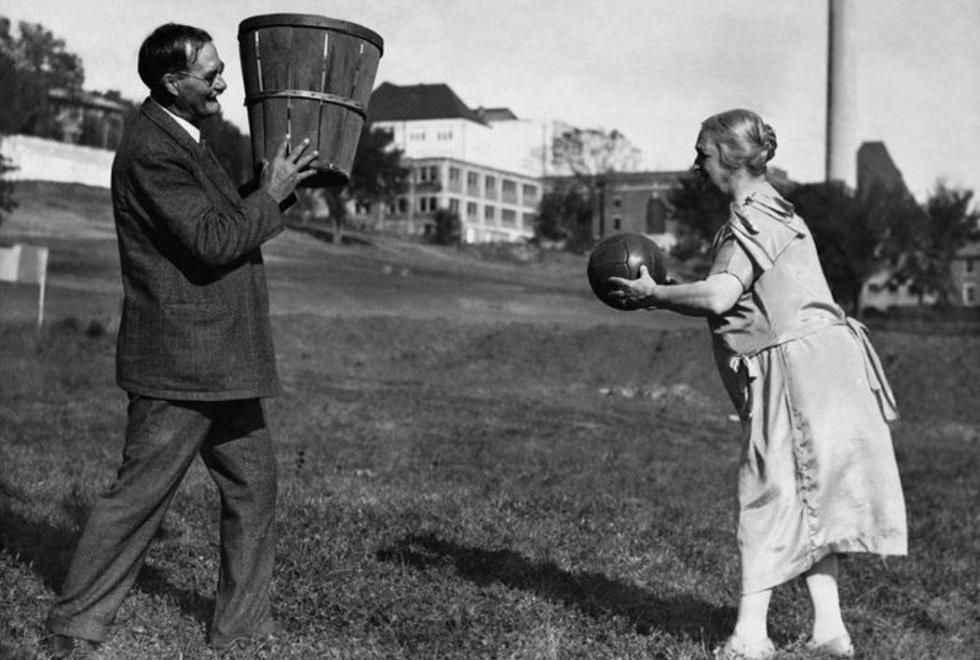
\includegraphics[width=0.3\textwidth]{imagenes/historia_baloncesto.jpg}
    \label{fig:hist_bskb}
\end{wrapfigure}

El baloncesto es un deporte de equipo que se originó en 1891, por James Naismith, profesor de educación física en la escuela YMCA de Springfield, Massachusetts, Estados Unidos.

James buscaba idear un deporte que sus alumnos pudieran practicar bajo techo, pues los duros inviernos en Massachusetts dificultaban la realización de ejercicio al aire libre, por lo que inventó el baloncesto utilizando unas cajas de melocotones y unos balones. 

Con el paso de los años, este deporte, que empezó como actividad de colegio, ha ido evolucionando mucho, añadiendo más reglas, conceptos nuevos, límites de números de jugadores, se ha determinado tiempos de juego, las canastas tienen un valor distinto según la distancia, etc.

Actualmente, las normas más básicas de este deporte son:
  
\begin{itemize}

  \item En las ligas superiores, hay un total de 4 cuartos de 10 minutos y pueden estar en pista 5 jugadores por equipo.
  \item No te puedes desplazar con la pelota en las manos, es obligatorio botar con una mano (si no será una infracción y conllevará la perdida de pelota y saque de banda del equipo rival).
  \item Cada jugador puede realizar hasta un total de 5 faltas, que será penalizado con un saque de banda o con un tiro libre (dependerá de la situación). El jugador que realiza 5 faltas será expulsado del partido.
  \item El objetivo es encestar el máximo de puntos posibles, teniendo en cuenta que pueden sumar 1, 2 o 3 puntos, según la distancia.

\end{itemize}

\clearpage

\subsection{Conceptos y definiciones básicas del baloncesto:}

Para que podamos entender a que nos referimos en este trabajo, es necesario comprender unos conceptos básicos de vocabulario. Tendremos en cuenta los conceptos que se necesitan para realizar la valoración del jugador y/o del equipo que se utilizan en las estadísticas federadas.

\begin{itemize}

\item Puntos: Acumulación de canastas encestadas multiplicadas por su valor, que cada  jugador y/o equipo realiza durante el partido
\item Minutos: Número de minutos que el jugador está en pista
\item Falta: Acción en la que un defensor bloquea el avance de su rival sin tener control de balón o de manera no reglamentaria (empujar, agarrar...)
\item Pérdidas de balón: cuando un equipo pierde el control del balón y pasa a ser del equipo rival.
\item Rebotes: Recuperación de pelota después de que el tiro sea ejecutado, pero no haya encestado.
\item Recuperación de balón: Cuando un equipo consigue robar el balón al equipo rival.
\item Asistencia: Es un pase a un jugador que se encuentra en una posición de ventaja o que le ayuda a conseguir una canasta sin hacer ningún bote.
\item Tapón: Bloqueo de un tiro en el aire.

\end{itemize}

\section{Posibles análisis realizables en el baloncesto}

Viendo la gran cantidad de datos que se pueden extraer de cada partido (y de cada equipo), se han ido creando análisis que recogen estos datos y los analizan para ayudarnos a identificar y desarrollar hipótesis sobre cada jugador y/o equipo.

\subsection{Boxscore}

El primer análisis que se hizo fue un \emph{Box Score} (Caja de puntuación) donde se recopilaba únicamente los puntos de cada jugador según el valor de esta y las faltas realizadas. Posteriormente, se fue mejorando añadiendo conceptos como rebotes, tapones, perdidas de balón, recuperaciones de balón... Y se añadió el estadístico (que acutalmente es por defecto) que se realiza a partir de todos estos datos: \emph{Valoración} (en inglés PIR, \emph{Performance Index Rating}) que engloba todo lo básico que pasa en el partido de manera individual y que, cuanto más positivo, mejor. Este estadístico se calcula utilizando la siguiente fórmula:
  
\begin{equation} \label{eq1}
  \begin{split}
  PIR = & (Puntos + Rebotes + Asistencias + Robos + Tapones + Faltas Recibidas) - \\
  & (Tiros de Campo Fallados + Tiros Libres Fallados + Tapones Recibidos + Pérdidas + Faltas Realizadas)
  \end{split}
\end{equation}

\centerline{(en el \hyperref[sec:Annexo1]{Annexo 1} encontraréis la descripción de cada variable)}

\vspace{0.2cm}

Posteriormente, se añadió la variable "Más/Menos" (\emph{P/M, Plus/Minus}) que tiene que ver con la diferencia de puntos en el marcador durante el tiempo que el jugador esté en pista. Esta variable sirve para ver la contribución de los jugadores cuando están en pista. Todos los jugadores parten inicialmente con un 0, y según van entrando y saliendo de la pista, esta variable se va actualizando. Por ejemplo, los jugadores que son del quinteto inicial, empiezan con el marcador 0 - 0, y un $P/M = 0$. Si en el minuto 5, se substituye un jugador en cancha del equipo local (J1) por otro que está descansando (J2), y el marcador va 12 - 7, el $P/M$ del J1 pasará a ser $+5$. Y si al cabo de 3 minutos, se sustituye el J2 por otro (J3) y el marcador ahora va 20 - 9, el $P/M$ del J2 será $+6$ ($(20-12) - (9-7) = 8 - 2 = +6$).

\begin{figure}[H]
\centering
\begin{minipage}{.5\textwidth}
\centering
\captionsetup{width=.8\linewidth}
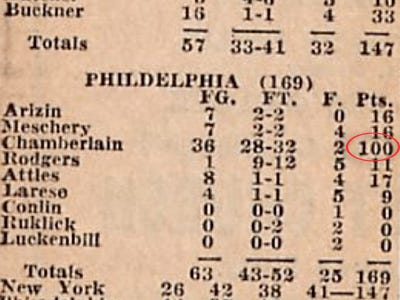
\includegraphics[width=.8\linewidth]{imagenes/BoxScore1962.jpg}
\captionof{figure}{Boxscore del partido de la NBA de Philadelphia Warriors contra New York Knicks, del 2 de Marzo de 1962}
\label{fig:BoxScore1962}
\end{minipage}%
\begin{minipage}{.5\textwidth}
\centering
\captionsetup{width=.8\linewidth}
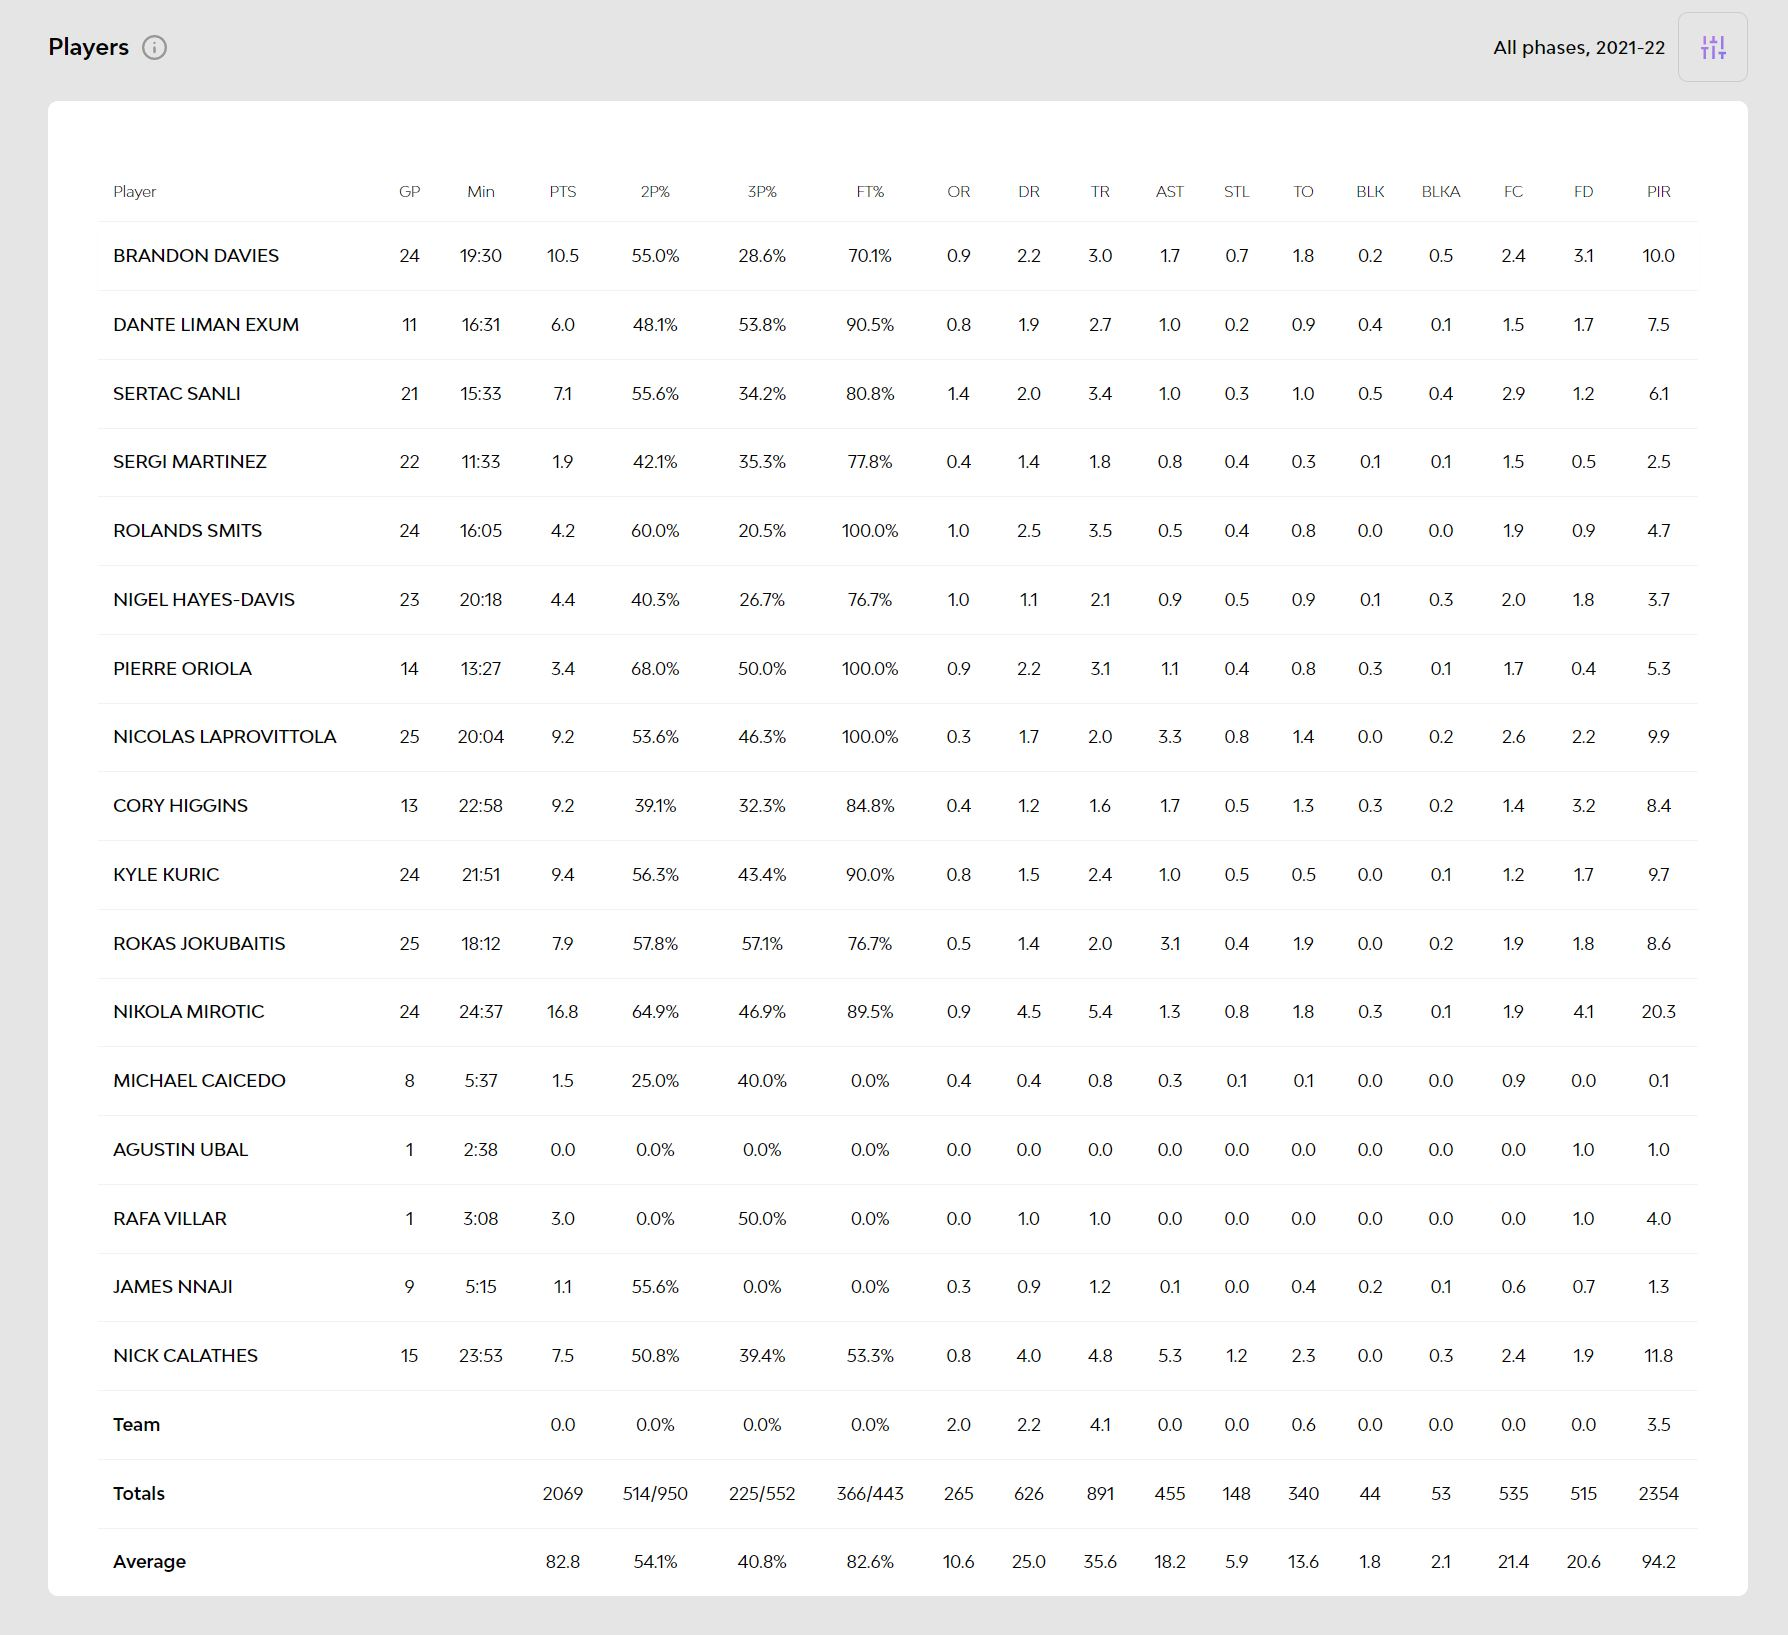
\includegraphics[width=.7\linewidth]{imagenes/BoxScore2022.jpg}
\captionof{figure}{Boxscore del partido de la Euroliga de Real Madrid contra FC Barcelona, del 11 de Febrero del 2022}
\label{fig:BoxScore2022}
\end{minipage}
\end{figure}

Aunque un \emph{Box Score} es muy útil para realizar análisis básicos, ya que es muy visual y cualquier persona sin la necesidad de muchos recursos puede analizar y predecir ciertos valores, pero estadísticamente perdemos una parte importante de la información de los datos, puesto que no nos los muestra progresivamente, sino que nos da los valores acumulados al final del tiempo establecido, y muchas veces contiene información engañosa, especialmente en las estadísticas defensivas.

Por lo que, para el desarrollo temporal del partido y para conocer cierta información de equipo que piden entrenadores y clubs, no nos sirve (como por ejemplo la eficacia de los quintetos, el desarrollo del marcador o de cualquier otra variable del equipo entero durante un tiempo determinado del partido, etc.)



\subsection{Play-by-play}

\begin{wrapfigure}{r}{0.4\linewidth}
    \centering
    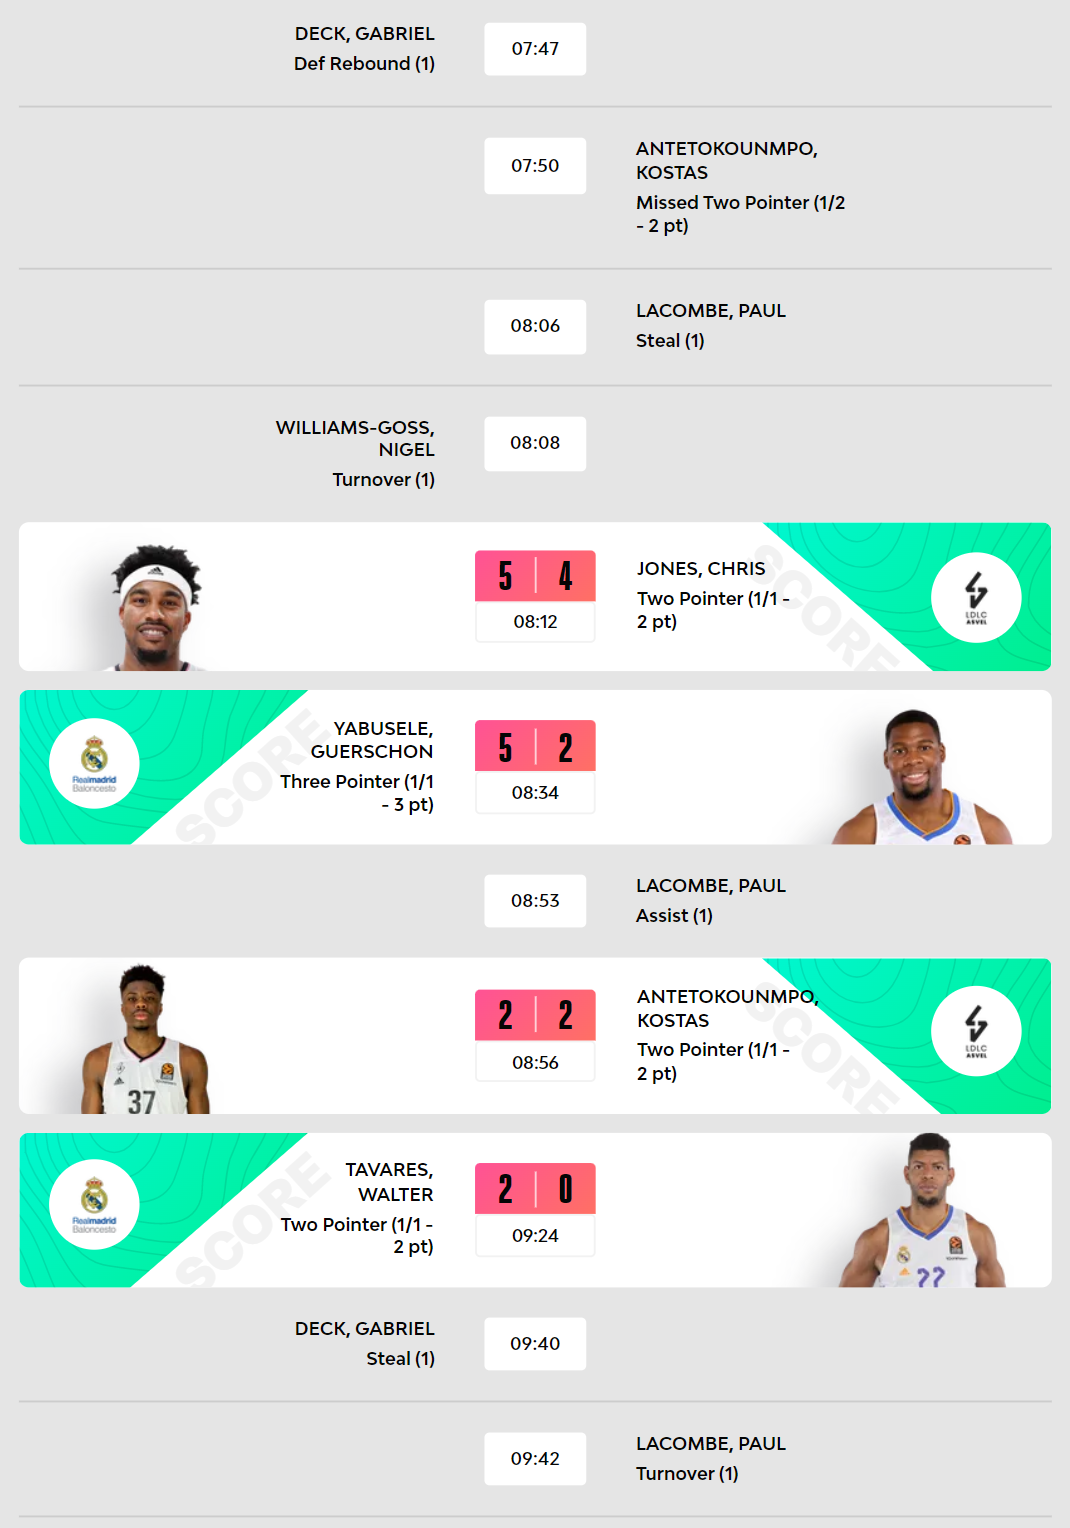
\includegraphics[width=0.4\textwidth]{imagenes/PBP_RM.png}
    \captionsetup{width=.9\linewidth}
    \captionof{figure}{\emph{Play by play} del partido de la Euroliga de Real Madrid contra LDLC Asvel, del 17 de Marzo del 2022. Se lee de abajo hacia arriba.}
    \label{fig:PBP_RM}
\end{wrapfigure}

Este tipo de recogida de información se creo para solucionar el problema que teniamos con el \emph{Box Score}. Los datos de \emph{Play-by-Play (PBP)} han sido la fuente principal de muchas estadísticas avanzadas, como el más-menos ajustado, que se desarrollará en este trabajo.

\emph{Play-by-Play} proporciona una transcripción del juego en un formato de eventos individuales. Los datos típicos de jugada por jugada deben tener la siguiente información:
  
  \begin{itemize}
\item El tiempo de la posesión
\item El jugador que inició la posesión (en caso de robo o rebote defensivo)
\item El jugador contrario que inició la posesión (en caso de un tiro fallado o pérdida de balón), incluida la ubicación en el piso desde donde se realizó el tiro y algunos otros identificadores únicos que usamos para clasificar el tipo de posesión.
\end{itemize}

Este tipo de análisis se inicializaron en 2007 para la Euroliga (principal competición europea de baloncesto) y en 2012 para la Eurocopa (competición internacional de segundo nivel).

\clearpage

\subsection{Shot-charts}

Este tipo de análisis es de los más visuales, ya que se realiza de una manera muy sencilla: se tiene como plantilla el dibujo de una pista de baloncesto de manera vectorial, y se va colocando cada tiro realizado en la posición del tiro, el jugador y si se encesta o no. De forma general se hace escribiendo el número del jugador en la posición des de donde se ejecuta el tiro, y si encesta, se hace un círculo alrededor del número.

El \emph{Shot-Charts}, proporciona un output visual muy fácil de interpretar, ya que es se parece a un mapa de calor y, por lo tanto, podemos observar de una manera muy rápida des de que zonas de la pista es más efectivo el equipo y/o el jugador.

Una vez realizado, podemos obtener con facilidad el porcentaje de acierto del equipo y/o el jugador, o incluso, determinar el porcentaje de acierto por zonas.

De este análisis, es frecuente encontrar variantes: mapa de calor del equipo, mapa de porcentajes de aciertos por zonas de la pista...

\subsection{Graphic Stats}




\clearpage

\section{Estadístico Más/Menos (\emph{Plus/Minus})}

\subsection{Normal Plus Minus, PM}

\subsection{Adjusted Plus Minus, APM}

\subsection{Regularized Adjusted Plus/Minus, RAPM}

\subsection{Real Plus-Minus, RPM}

\clearpage

\addcontentsline{toc}{section}{Referencias}

\begin{thebibliography}{X}
	\bibitem{RAPM} \textsc{Joseph Sill}, \textit{Improved NBA Adjusted +/- Using Regularization and Out-of-Sample Testing}, PDF, 6 Marzo 2010.
	
	\bibitem{HappyGH} \textsc{Happy Git}, \textit{Let’s Git started}, url: \url{https://happygitwithr.com/index.html}, .
\end{thebibliography}

\clearpage

\section{Annexo}

\subsection{Descripción de las variables} \label{sec:Annexo1}

\begin{itemize}
\item MIN (\emph{Minutes}): Minutos totales jugados
\item PTS (\emph{Points}): Puntos totales realizados
\item 2FGA (\emph{2-point Field Goals Attempted}): Número de canastas de 2 puntos intentadas
\item 2FGM (\emph{2-point Field Goals Made}): Número de canastas de 2 puntos anotadas
\item 3FGA (\emph{3-point Field Goals Attempted}): Número de canastas de 3 puntos ("triples") intentadas
\item 3FGM (\emph{3-point Field Goals Made}): Número de canastas de 3 puntos ("triples") anotadas
\item FTA (\emph{Free Throws Attempted}): Número de tiros libres intentados
\item FTM (\emph{Free Throws Made}): Número de tiros libres anotados
\end{itemize}

\clearpage

\subsection{Código R} \label{sec:Annexo2}

\begin{Schunk}
\begin{Sinput}
> library(readr)
> library(dplyr)
> library(ggplot2)
> library(here)
> library(tidyverse)
\end{Sinput}
\end{Schunk}

\begin{Schunk}
\begin{Sinput}
> pbp2018 <- read.csv(file="pbp2018.csv", head=TRUE, sep=",")
> names(pbp2018)
\end{Sinput}
\begin{Soutput}
 [1] "season"         "game_code"      "play_number"    "team_code"     
 [5] "player_name"    "play_type"      "time_remaining" "quarter"       
 [9] "points_home"    "points_away"    "play_info"      "seconds"       
[13] "home_team"      "away_team"      "home"           "team_name"     
[17] "last_ft"        "and1"           "home_player1"   "home_player2"  
[21] "home_player3"   "home_player4"   "home_player5"   "away_player1"  
[25] "away_player2"   "away_player3"   "away_player4"   "away_player5"  
[29] "lineups"       
\end{Soutput}
\end{Schunk}

Se encontraron errores en la extracción de las alineaciones. Corrección:

\begin{Schunk}
\begin{Sinput}
> pbp_2018 <- read_csv("pbp2018.csv")
> ## Check how many rows are affected by this
> bad_lineups <- pbp_2018 %>%
+   select(matches("_player[1-5]")) %>%
+   apply(1, function(x) max(table(x)) > 1)
> pbp_bad <- pbp_2018 %>%
+   filter(bad_lineups)
> pbp_bad %>%
+   select(season, game_code, play_number, play_type, away_player4, away_player5)
\end{Sinput}
\begin{Soutput}
# A tibble: 10,260 x 6
   season game_code play_number play_type away_player4 away_player5
    <dbl>     <dbl>       <dbl> <chr>     <chr>        <chr>       
 1   2018         2          93 IN        TOMIC, ANTE  TOMIC, ANTE 
 2   2018         2          94 OUT       TOMIC, ANTE  TOMIC, ANTE 
 3   2018         2          95 OUT       TOMIC, ANTE  TOMIC, ANTE 
 4   2018         2          96 IN        TOMIC, ANTE  TOMIC, ANTE 
 5   2018         2          97 OUT       TOMIC, ANTE  TOMIC, ANTE 
 6   2018         2          98 IN        TOMIC, ANTE  TOMIC, ANTE 
 7   2018         2          99 OUT       TOMIC, ANTE  TOMIC, ANTE 
 8   2018         2         100 FTM       TOMIC, ANTE  TOMIC, ANTE 
 9   2018         2         101 FTM       TOMIC, ANTE  TOMIC, ANTE 
10   2018         2         116 AST       KURIC, KYLE  KURIC, KYLE 
# ... with 10,250 more rows
\end{Soutput}
\begin{Sinput}
> ## Solución
> source(here("R", "fix-lineups.R"))
> ## Function fix_lineups() only takes data from a single game,
> ## so I split the data and apply the function to each splitted data frame.
> pbp_2018_fixed <- split(pbp_2018, factor(pbp_2018$game_code)) %>%
+   map_df(fix_lineups)
> ## Check that this has been fixed
> pbp_2018_fixed %>%
+   select(matches("_player[1-5]")) %>%
+   apply(1, function(x) max(table(x)) > 1) %>%
+   sum()
\end{Sinput}
\begin{Soutput}
[1] 0
\end{Soutput}
\end{Schunk}

\subsubsection{MAS/MENOS Clásico}
    
\begin{Schunk}
\begin{Sinput}
> df <- pbp_2018_fixed
> # Lista de jugadores:
> players <- df %>% 
+   select(matches("player_name")) %>%
+   arrange(player_name) %>% 
+   unique
> num_players <- dim(players)[1]    # Numero de jugadores
> unique(df$play_type)              # Tipos de acciones
\end{Sinput}
\begin{Soutput}
 [1] "BP"      "TPOFF"   "2FGM"    "2FGA"    "DRB"     "3FGA"    "ORB"    
 [8] "CPF"     "RPF"     "FTM"     "TOV"     "STL"     "3FGM"    "AST"    
[15] "OF"      "TOUT"    "IN"      "OUT"     "FTA"     "EP"      "RBLK"   
[22] "BLK"     "EG"      "TOUT_TV" "CMU"     "C"       "CMT"     "B"      
[29] "AS"      "RV"      "CMD"     "D"      
\end{Soutput}
\begin{Sinput}
> names(df)                         # Variables BBDD
\end{Sinput}
\begin{Soutput}
 [1] "season"         "game_code"      "play_number"    "team_code"     
 [5] "player_name"    "play_type"      "time_remaining" "quarter"       
 [9] "points_home"    "points_away"    "play_info"      "seconds"       
[13] "home_team"      "away_team"      "home"           "team_name"     
[17] "last_ft"        "and1"           "home_player1"   "home_player2"  
[21] "home_player3"   "home_player4"   "home_player5"   "away_player1"  
[25] "away_player2"   "away_player3"   "away_player4"   "away_player5"  
[29] "lineups"       
\end{Soutput}
\begin{Sinput}
> df_pbp <- df %>% 
+   select(season, game_code, quarter, points_home, points_away, matches("_player[1-5]"))
> df_pbp$PM_Home <- df_pbp$points_home - df_pbp$points_away
> df_pbp$PM_Away <- -df_pbp$PM_Home
> names(df_pbp)                     # Variables finales BBDD
\end{Sinput}
\begin{Soutput}
 [1] "season"       "game_code"    "quarter"      "points_home"  "points_away" 
 [6] "home_player1" "home_player2" "home_player3" "home_player4" "home_player5"
[11] "away_player1" "away_player2" "away_player3" "away_player4" "away_player5"
[16] "PM_Home"      "PM_Away"     
\end{Soutput}
\end{Schunk}
      
      
\subsubsection{MAS/MENOS AJUSTADO, \emph{APM}}
    
\begin{Schunk}
\begin{Sinput}
>       
\end{Sinput}
\end{Schunk}

\end{document}
